\documentclass[11pt]{article}
\usepackage[T1]{fontenc}
\usepackage[utf8]{inputenc}
\usepackage{lmodern}
\usepackage[margin=1.03in]{geometry}
\usepackage{amsmath,amssymb,amsthm,mathtools,mathrsfs,xcolor}
\usepackage{microtype,enumitem,tikz}
\usetikzlibrary{arrows.meta,positioning,calc}
\PassOptionsToPackage{hyphens}{url}
\usepackage{hyperref,bookmark}
\hypersetup{colorlinks=true,linkcolor=blue!45!black,citecolor=blue!45!black,urlcolor=blue!45!black,pdftitle={A Counterexample to Kaplansky's Direct-Finiteness Conjecture in Odd Characteristic},pdfauthor={OpenAI}}
\input{glyphtounicode-cmex.tex}
\pdfgentounicode=1
\pdfinfoomitdate=1
\pdftrailerid{}
\pdfsuppressptexinfo=15
\newtheorem{theorem}{Theorem}[section]
\newtheorem{proposition}[theorem]{Proposition}
\newtheorem{lemma}[theorem]{Lemma}
\newtheorem{corollary}[theorem]{Corollary}
\theoremstyle{remark}
\newtheorem{remark}[theorem]{Remark}
\numberwithin{equation}{section}
\newcommand{\F}{\mathbb F}
\newcommand{\Mat}{\operatorname{Mat}}
\newcommand{\diag}{\operatorname{diag}}
\newcommand{\im}{\operatorname{im}}
\newcommand{\rank}{\operatorname{rank}}
\newcommand{\id}{\mathrm{id}}
\newcommand{\supp}{\operatorname{supp}}
\setlength{\emergencystretch}{1.5em}
\setlist[enumerate]{itemsep=3pt,topsep=5pt}
\title{A Counterexample to Kaplansky's Direct-Finiteness Conjecture in Odd Characteristic}
\author{OpenAI}
\date{September 26, 2026}
\begin{document}
\maketitle
\begin{abstract}
We construct a counterexample to Kaplansky's direct-finiteness conjecture in odd characteristic. For one specified odd prime $p$, we obtain a field $K$ of order $p^4$, a finitely generated group $G$ containing torsion, and finite sums $a,b\in K[G]$ with $ab=1$ but $ba\ne1$. The same elements define a cellular automaton on $K^G$ that is injective but not surjective.
\end{abstract}
\section{Introduction}
\label{op:introduction}

A group algebra $K[G]$ consists of finite sums $\sum_g c_g g$, with
$c_g\in K$, multiplied by the group law and bilinearity. A unital ring is
\emph{directly finite} when $ab=1$ implies $ba=1$; it is \emph{stably
finite} when this implication holds in every finite square matrix ring.
Kaplansky's direct-finiteness conjecture asks whether $K[G]$ is directly
finite for every field $K$ and every group $G$, including groups with
torsion. The result here is a negative answer in one specified
odd characteristic.

\begin{theorem}\label{op:main}
Put
\[
 m=\binom{1200}{600},\qquad
 p=\min\{h\in\mathbb Z:h>1,\ h\mid(m!)^2+1\}.
\]
Then $p$ is an odd prime. There are a specified field $K$ of order $p^4$,
a specified finitely generated group $G$ containing torsion, and specified
finite sums $a,b\in K[G]$ satisfying $ab=1$ and $ba\ne1$.
\end{theorem}

The word ``specified'' refers to finite formulas and choices in ordered
finite sets. The field is a quadratic tower, the group is built from
finitely many finite groups and explicit identifications, and the sums
are defined without solving the word problem of that group. The
construction is not claimed to have been evaluated as a practical
computation. It concerns the displayed prime, not every odd prime.

\paragraph{The finiteness problem.}
For finite $G$, the algebra and all its finite matrix rings are
finite-dimensional over $K$. A one-sided inverse between their left
multiplication operators is therefore two-sided. This argument works even
when the characteristic divides $|G|$. The difficulty for an infinite
group is to obtain a corresponding conclusion from finite support alone.

Kaplansky proved stable finiteness in characteristic zero using finite
von Neumann algebras, and asked whether the one-sided-inverse property
persists in positive characteristic~\cite[pp.~122--123]{Kaplansky1972}.
Ara, O'Meara, and Perera proved stable finiteness for free-by-amenable
groups over arbitrary division rings~\cite{AraOMearaPerera2002}.
Elek and Szab\'o~\cite[Corollary~4.7]{ElekSzabo2004} established the
same conclusion for all sofic groups. Such groups admit finite
permutation models that approximate multiplication while keeping
distinct elements separated.
These theorems are constraints on the example, not hypotheses about its
group. In particular, Elek--Szab\'o's theorem implies, after the scalar
construction is completed, that $G$ cannot be sofic.

A separate characteristic-two construction uses incidence structures,
polynomial pairings, a planar group-embedding argument, and character
packing~\cite[Theorem~1.1]{OpenAICharacteristicTwo2026}.
The construction here has a different local mechanism. A high-degree
subspace of a modular translation representation is annihilated on one
side; a weighted pairing gives a compatible annihilation on the other.
The characteristic-two theorem is not an input to this odd-prime
argument, and the two methods retain distinct coefficient hypotheses.

\paragraph{The two quantities that must be compared.}
A matrix $F$ \emph{fits} a simple graph when $F_{ii}=1$ and $F_{ij}=0$
for distinct nonadjacent vertices. We use a triangle-free graph on $m$
vertices and a specified factorization
\[
 F_{ij}=\sum_{T\in\mathcal T}\alpha_i(T)\beta_j(T),\qquad
 |\mathcal T|=t,\qquad \frac{t}{m}<\frac1{100}.
\]
This is an explicit threshold-Kneser instance of the polynomial
constructions of Haviv and Golovnev--Haviv
\cite[Proposition~13]{Haviv2018Theta}
\cite[Theorem~3.2 and Lemma~3.5]{GolovnevHaviv2022}, whose polynomial
ancestry includes Alon--Babai--Suzuki~\cite{AlonBabaiSuzuki1991}.
Low-rank fitting matrices also give storage-code recovery equations.
The triangle-free constructions of Barg--Z\'emor, Huang--Xiang, and
Barg--Schwartz--Yohananov provide related context
\cite{BargZemor2022,HuangXiang2023,BargSchwartzYohananov2024}.
Their results are not used to supply a group-algebra idempotent.

At every vertex we use a copy of a finite group $H$ and an idempotent
$e\in K[H]$. Write $w=|H|$ and $d=\dim_K eK[H]$, the rank of left
multiplication by $e$ on the regular representation. The second quantity
is
\[
 \frac d w>\frac1{96}.
\]
The idempotents satisfy a directed condition: after identifying certain
cyclic subgroups at adjacent vertices, $e_i e_j=0$ for every edge with
$i<j$. There is no assertion about the reverse product. The asymmetry is
what allows a triangular calculation to combine the two strict bounds.

The characteristic-dependent construction appears in
Section~\ref{op:modular-section}. High augmentation degree gives the
annihilated columns, in the elementary abelian setting of
Jennings' theory~\cite{Jennings1941}. A diagonal weighted Gram determinant
and Schwartz's grid bound~\cite[Lemma~1 and Corollary~1]{Schwartz1980},
with related polynomial-identity work of Zippel~\cite{Zippel1979}, supply
enough nondegenerate pairings. Fourier character orbits turn these
projections into actual elements of $K[H]$. The full algebra need not
be semisimple; only its prime-to-$p$ normal abelian subgroup is
diagonalized, in the character-orbit setting of
Clifford~\cite{Clifford1937Announcement}.

\paragraph{From the comparison to scalar elements.}
The proof has three transitions that numerical rank inequalities alone
cannot justify. First, the quotient identifying the cyclic subgroups must
retain the finite vertex groups. Its injectivity proof uses the
$C(4)$--$T(4)$ graphical-complex mechanism described by
Prytu\l a~\cite[Section~8]{Prytula2024}: local short-word restrictions and
triangle-freeness rule out a spherical map with exactly one nontrivial
face. Ordinary graph-of-groups normal form does not by itself establish
this first quotient's injectivity. Section~\ref{sec:gluing} proves it
locally, including the reductions for loops and bridges.

Second, regular ranks must become identities over the same ring. A
further group enlargement $G_1$ has a nonzero central idempotent $f$ in
$R=K[G_1]$. In the ring $S=fR$, whose identity is $f$, the elements
$P_i=fe_i$ admit rectangular matrices
\[
 J_i\in\Mat_{w\times d}(S),\qquad
 Y_i\in\Mat_{d\times w}(S),\qquad
 Y_iJ_i=fI_d,\quad J_iY_i=P_iI_w.
\]
The finite-group blocks in this step have elementary abelian $p$-group
stabilizers, possibly nontrivial and nonnormal. Their group algebras have
nilpotent augmentation ideals, and a finite
change of basis proves exact integer rank identities before coordinates
are paired. Section~\ref{sec:sector} gives the full construction of these
matrices, with their entries in explicitly attached finite subgroups.

Third, a matrix counterexample does not yet give two scalar elements of
the same group algebra. In Section~\ref{op:compression-section}, the
fit and the ordered zero products produce a split injection
\[
 S^{md}\longrightarrow S^{wt}\longrightarrow S^{md},
 \qquad wt<md,
\]
whose composite is the identity. We derive square matrices with a
one-sided inverse and certify the reverse defect by a nonzero kernel
vector. Section~\ref{op:scalar-section} then implements the finite-factor
reduction of Dykema--Juschenko~\cite[Lemma~2.1 and Theorem~2.2]{DykemaJuschenko2015}.
A finite Heisenberg group gives explicit matrix units, their linear
independence makes the encoding injective, and a complementary idempotent
restores the full scalar identity. The shift and modulation model is
classical~\cite[Section~1.2]{GurevichHadani2009}; the composite cyclic
order and finite coefficient field used here are checked directly.

\paragraph{The dynamical consequence.}
A configuration over a finite alphabet $A$ is any function $G\to A$.
A cellular automaton has one finite memory set $E\subset G$ and one
rule applied to $(x(gu))_{u\in E}$ at every $g$. A group is
\emph{surjunctive} when every injective such automaton, over every finite
alphabet, is surjective. Gottschalk proposed this for all groups
\cite{Gottschalk1973}; Gromov and Weiss proved it for sofic groups
\cite{Gromov1999,Weiss2000}. The group-ring connection is recorded by
Elek--Szab\'o and developed in the linear theory of
Ceccherini-Silberstein--Coornaert
\cite{ElekSzabo2004,CSCCoornaert2006}. Phung proved stable finiteness
over every field for surjunctive groups~\cite[Theorem~B]{Phung2023};
subsequent proofs and extensions include~\cite{CSCPhungGroup2025,CSCPhungMonoid2025}.

Section~\ref{op:cellular-section} gives the elementary transfer with its
actual multiplication convention. The coefficients of $b$ define an
injective automaton, those of $a$ give a left inverse, and a nonzero
coefficient of $ba-1$ specifies a missing point indicator. The argument
excludes preimages of arbitrary support. It is a consequence of the
scalar construction, not a further existence theorem.

All matrices below act on columns of free right modules. Matrix entries
therefore multiply coordinates on the left. Transpose is ordinary
transpose over $K$, with no involution. Cardinalities and dimensions in
rank comparisons are integers, not elements of the coefficient field.
For a positive integer $n$, write $[n]=\{1,\ldots,n\}$.

\section{The field, the graph, and the local group}
\label{op:finite-section}

We first construct the finite data. This fixes every coefficient field
and denominator before the modular argument begins.

\begin{lemma}\label{op:field}
For $m,p$ in Theorem~\ref{op:main}, $p>m$ is an odd prime and $-1$
is a square in $\F_p$. If $\eta$ is a nonsquare in $\F_p^*$, then
\[
 K_0=\F_p[\xi]/(\xi^2-\eta),\qquad
 K=K_0[\nu]/(\nu^2-\xi)
\]
are quadratic field extensions, so $|K|=p^4$.
\end{lemma}
\begin{proof}
A least divisor greater than one of an integer is prime: any nontrivial
proper divisor of a composite least divisor would be smaller. If $p\le m$,
then $p$ divides both $m!$ and $(m!)^2+1$, which is impossible. Hence
$p>m>600$, and the defining divisibility gives $(m!)^2=-1$ in $\F_p$.
There are nonsquares because each nonzero square has exactly two square
roots. The first quotient is therefore a quadratic field. The conjugate
of $\xi$ is $-\xi$, so its norm is $-\eta$. Since $-1$ is square,
$-\eta$ is nonsquare. A square in $K_0$ would have square norm, proving
that $\xi$ is nonsquare and that the second quotient is a field.
\end{proof}

Choose the least nonsquare using representatives $0,\ldots,p-1$; order
$K$ by its coefficients in $(1,\xi,\nu,\xi\nu)$. Put $M=p^4-1$ and
choose the least element $\zeta\in K^*$ of order $M$. This element
exists: if $b$ is the least common multiple of all orders in $K^*$,
then $b\mid M$, while the root bound for $X^b-1$ gives $M\le b$.
For each prime-power factor of $b$, an appropriate power of one element
has that exact order. Multiplying the resulting commuting elements of
coprime orders gives order $b=M$. In particular, $M$ and all its powers
are invertible in $K$.

Use natural orders on integer indices, increasing-list lexicographic
orders on subsets, and lexicographic orders on tuples and finite function
tables. Order characters of $(\mathbb Z/M\mathbb Z)^D$ by their exponent
lists on the ordered coordinate generators. These conventions specify
the finite choices below.

Let $I_1,\ldots,I_m$ be the $600$-subsets of $[1200]$ in order. Join
distinct $i,j$ in $\Gamma$ exactly when $|I_i\cap I_j|<200$. Put
\[
 \mathcal T=\{T\subseteq[1200]:|T|\le400\},\qquad
 t=\sum_{j=0}^{400}\binom{1200}{j}.
\]

\begin{proposition}\label{op:graph}
The graph $\Gamma$ is triangle-free and has a specified fitting
factorization $F_{ij}=\sum_{T\in\mathcal T}\alpha_i(T)\beta_j(T)$
over $\F_p$ with $t/m<1/100$.
\end{proposition}
\begin{proof}
Three pairwise adjacent sets would have union of size at least
$3\cdot600-3\cdot199=1203$, exceeding $1200$. To construct the fit, let
$\alpha_i(T)=1$ when $T\subseteq I_i$, and zero otherwise. Define
$\beta_j(T)$ as the coefficient of $\prod_{x\in T}X_x$ obtained by
expanding
\[
 Q_j(X)=\prod_{k=200}^{599}
       \frac{\sum_{x\in I_j}X_x-k}{600-k}
\]
and replacing every positive exponent in each monomial by one. All
denominators are in $\{1,\ldots,400\}$, hence invertible. This replacement
preserves evaluations on zero-one vectors and does not increase degree.
Thus
\[
 F_{ij}=\prod_{k=200}^{599}\frac{|I_i\cap I_j|-k}{600-k}.
\]
It equals one for $i=j$. For distinct nonneighbors the intersection
size lies between $200$ and $599$, so one factor is zero. This is the
threshold-Kneser polynomial specialization of
\cite[Proposition~13]{Haviv2018Theta}
\cite[Theorem~3.2]{GolovnevHaviv2022}.

The binomial coefficients increase up to index $400$. Consequently
\[
 \frac{t}{m}
 \le401\prod_{u=401}^{600}\frac{u}{1201-u}
 \le401(5/7)^{100}<\frac1{100}.
\]
In the second inequality the first hundred factors are at most
$500/701<5/7$ and the rest are at most one. The last inequality follows
from $(5/7)^3<1/2$ and $40100<2^{33}$.
\end{proof}

For the local algebra define the additive group $P=(\F_p)^3$, the
function group $A_0=(\mathbb Z/M\mathbb Z)^P$, and
\[
 H=A_0\rtimes P,\qquad
 (a,s)(a',s')=(a+s\cdot a',s+s'),\qquad
 (s\cdot a)(x)=a(x-s).
\]
Its order is $w=M^{p^3}p^3$. Let $c\in A_0$ have value one at zero and
zero elsewhere, and put
\[
 u(s)=(0,s),\quad U=u(P),\qquad
 v(s)=cu(s)c^{-1},\quad V=cUc^{-1}.
\]
The coordinate formula $v(s)=(c-s\cdot c,s)$ gives $U\cap V=\{1\}$,
because $c-s\cdot c\ne0$ when $s\ne0$. We next construct an idempotent
with incoming annihilation by $U$ and outgoing annihilation by $V$.

\section{Large idempotents with ordered annihilations}
\label{op:modular-section}

The graph has supplied the ratio $t/m<1/100$. Our present objective is
an idempotent in the finite group algebra $K[H]$ whose regular rank
fraction exceeds $1/96$. It must also have two prescribed annihilations,
on opposite sides. Here
\[
 \ell=(p-1)/2,\qquad D=3(p-1),\qquad w=|H|.
\]
The \emph{regular rank} of $e\in K[H]$ means
$\dim_K eK[H]$, the dimension of the image of left multiplication.
Although this map multiplies on the left, its image is a right ideal.

\begin{proposition}\label{op:modular}
There is a specified idempotent $e\in K[H]$ satisfying, for every $s\in P$,
\[
 (u(s)-1)^\ell e=0,\qquad e(v(s)-1)^\ell=0.
\]
Its regular rank $d$ satisfies $d/w>1/96$. Its coefficients are obtained
by finite operations in the specified field $K$.
\end{proposition}

\subsection{The annihilated column space}

On $K^P$, let $\mathbf e_x$ be the standard basis and
$L_s\mathbf e_x=\mathbf e_{s+x}$. For the three standard generators
$\varepsilon_j$ of $P$ set $X_j=L_{\varepsilon_j}-I$. The $X_j$ commute,
and characteristic $p$ gives $X_j^p=0$. The vectors
\[
 X_1^{n_1}X_2^{n_2}X_3^{n_3}\mathbf e_0,
 \qquad 0\le n_1,n_2,n_3<p,
\]
are a basis. Indeed, every translation of $\mathbf e_0$ is a product of
powers of $I+X_j$ applied to $\mathbf e_0$, so the displayed family spans
$K^P$; its cardinality is the dimension $p^3$.

This is the elementary abelian augmentation filtration in the setting
studied by Jennings~\cite{Jennings1941}. Here the exact degree argument
can be given directly. Let $B$ have as columns the displayed basis
vectors with $n_1+n_2+n_3\ge D-\ell+1$, in order. For every $s$, the
matrix $L_s-I$ is a polynomial in the $X_j$ with zero constant term.
Multiplication by its $\ell$th power raises every column's total degree
to at least $D+1$. Such a monomial has an exponent at least $p$, so
vanishes. Applying the same assertion to $-s$ and transposing yields
\begin{equation}\label{op:B-annihilation}
 (L_s-I)^\ell B=0,\qquad B^{\mathsf T}(L_s-I)^\ell=0.
\end{equation}
The transpose identity uses $L_{-s}^{\mathsf T}=L_s$; no scalar
conjugation is present.

The columns are independent. Their number $h$ can be counted by setting
$a_j=p-1-n_j$: the new nonnegative indices have sum at most $\ell-1$.
Their individual upper bounds are automatic because $\ell-1<p$.
Stars and bars gives
\begin{equation}\label{op:h}
 h=\binom{\ell+2}{3},\qquad
 \frac{h}{p^3}=\frac{(p-1)(p+1)(p+3)}{48p^3}>\frac1{48}.
\end{equation}
For the strict inequality, the numerator minus $p^3$ is
$3p^2-p-3>0$ for $p\ge3$.

The same subspace is killed on the two sides in
Equation~\eqref{op:B-annihilation}, but an arbitrary projection onto it
need not give the outgoing conjugate annihilation. We therefore choose
the row factor by a diagonal weighted pairing.

\subsection{Many nonsingular diagonal pairings}

For a finite function group $A_*=(\mathbb Z/M\mathbb Z)^E$, its
characters $\chi:A_*\to K^*$ are all exponent lists of powers of
$\zeta$. Put
\begin{equation}\label{op:fourier}
 p_\chi^{A_*}=|A_*|^{-1}\sum_{a\in A_*}\chi(a)^{-1}a.
\end{equation}
The denominator is invertible. Reindexing the sum gives
$a p_\chi^{A_*}=\chi(a)p_\chi^{A_*}$. A nontrivial character has sum
zero, since translating its sum by an element on which it is nontrivial
multiplies it by a scalar different from one. It follows that
\[
 p_\chi^{A_*}p_\psi^{A_*}=\delta_{\chi\psi}p_\chi^{A_*},\qquad
 \sum_\chi p_\chi^{A_*}=1.
\]
For the last identity, sum coefficients over the independent character
exponents: every nonzero coordinate of a nonidentity element is detected
by a power of $\zeta$. Each idempotent is nonzero, there are $|A_*|$ of
them, and orthogonality makes them independent. They form a basis of
$K[A_*]$.

Specialize to $A_0$. Its character action is
$(s\lambda)(a)=\lambda((-s)\cdot a)$. Define
\[
 \chi_x=x\lambda,\qquad
 D_\lambda=\diag(\chi_x(c):x\in P),\qquad
 N_\lambda=B^{\mathsf T}D_\lambda^{-1}B.
\]
Call $\lambda$ admissible if its stabilizer in $P$ is trivial and
$N_\lambda$ is invertible. This condition is a finite test.

\begin{lemma}\label{op:good-count}
More than half of the $|A_0|=M^{p^3}$ characters are admissible.
\end{lemma}
\begin{proof}
For each nonzero $s\in P$, translation partitions $P$ into $p^2$ cycles
of length $p$. A character fixed by $s$ has constant exponent on each
cycle, so exactly $M^{p^2}$ characters are fixed. A union bound therefore
bounds the fraction with nontrivial stabilizer by
\[
 (p^3-1)M^{p^2-p^3}.
\]

Let $c_r$ be the coordinate generator at $r$. Since
$\chi_x(c)=\lambda(c_{-x})$, the diagonal entries of $D_\lambda^{-1}$
range independently over $K^*$ as $\lambda$ ranges over all characters.
For independent variables $\tau_x$, Cauchy--Binet gives
\begin{equation}\label{op:weighted-gram}
 Q(\tau):=\det\bigl(B^{\mathsf T}\diag(\tau_x)B\bigr)
 =\sum_{\substack{J\subseteq P\\|J|=h}}\det(B_J)^2\prod_{x\in J}\tau_x.
\end{equation}
Here $B_J$ consists of the indicated rows in their fixed order.
Some maximal minor is nonzero because $B$ has full column rank. The
monomials for distinct $J$ are distinct, so $Q$ is nonzero of total
degree $h$, even though the unweighted Gram matrix could be singular.

We use the polynomial grid estimate of
Schwartz~\cite[Lemma~1 and Corollary~1]{Schwartz1980}; see also the
related identity-testing method of Zippel~\cite{Zippel1979}. A nonzero
polynomial of total degree at most $a$ vanishes on at most an $a/M$
fraction of a product grid whose coordinate sets each have size $M$.
To prove this, induct on the number of variables. If the degree in the
last variable is $b$, its leading coefficient has degree at most $a-b$.
It vanishes at at most an $(a-b)/M$ fraction of the earlier choices.
For each remaining choice, the last-variable polynomial has at most
$b$ roots, contributing at most $b/M$. The sum proves the bound; the
constant case starts the induction.

Applying the estimate on $(K^*)^{p^3}$ to
Equation~\eqref{op:weighted-gram}, the singular-pairing fraction is at
most $h/M$. Both excluded fractions are strictly smaller than $1/4$:
\[
 \frac hM\le\frac{p^3}{p^4-1}<\frac14,\qquad
 (p^3-1)M^{-p^2(p-1)}\le\frac{p^3-1}{M}<\frac14.
\]
The estimates use $p>600$; for example,
$p^4-1-4p^3=p^3(p-4)-1>0$. Their union therefore excludes fewer than
half of the characters.
\end{proof}

Select the first admissible character from each $P$-orbit containing one,
and call the set of selected characters $\mathscr R$. Each selected
orbit is free, of size $p^3$. These orbits cover all admissible characters,
so
\begin{equation}\label{op:orbit-count}
 |\mathscr R|>\frac{|A_0|}{2p^3}.
\end{equation}
This argument does not need admissibility to be constant on an orbit.

\subsection{Realizing the projections in the group algebra}

Fix $\lambda\in\mathscr R$. For $x,y\in P$, define
\[
 E_{xy}^{\lambda}=p_{x\lambda}^{A_0}u(x-y).
\]
Conjugation gives $u(s)p_\chi^{A_0}u(s)^{-1}=p_{s\chi}^{A_0}$.
Fourier orthogonality and freeness of the orbit therefore imply
\[
 E_{xy}^{\lambda}E_{zt}^{\lambda}=\delta_{yz}E_{xt}^{\lambda}.
\]
Indeed the Fourier product can survive only when
$x\lambda=(x-y+z)\lambda$, which is equivalent to $y=z$.
Products between different orbits vanish. The sum
$q_\lambda=\sum_x p_{x\lambda}^{A_0}$ is central: it commutes with
$A_0$ and its summands are permuted by $P$. The basis
$p_{x\lambda}^{A_0}u(s)$ of its ideal is indexed equally by $(x,y)$
through $s=x-y$. Thus these units prove
\[
 q_\lambda K[H]\cong\Mat_{p^3}(K).
\]
This is an explicit character-orbit block, in the normal-subgroup
representation setting of Clifford~\cite{Clifford1937Announcement}.
It does not assert semisimplicity of the entire modular algebra.

On this block, the elements $u(s)$, $c$, and $v(s)$ act respectively by
\[
 L_s,\qquad D_\lambda,\qquad D_\lambda L_sD_\lambda^{-1}.
\]
For example, left multiplication by $u(s)$ shifts row $x$ to row $s+x$,
whereas $c$ multiplies row $x$ by $(x\lambda)(c)$.

Define a matrix and then a finite group-algebra element by
\begin{equation}\label{op:explicit-e}
 T_\lambda=BN_\lambda^{-1}B^{\mathsf T}D_\lambda^{-1},\qquad
 e=\sum_{\lambda\in\mathscr R}\sum_{x,y\in P}
       (T_\lambda)_{xy}E_{xy}^{\lambda}.
\end{equation}
The inverse exists by the selection criterion. Since
$B^{\mathsf T}D_\lambda^{-1}B=N_\lambda$, we have $T_\lambda B=B$
and $T_\lambda^2=T_\lambda$. Its image is exactly $\im B$, of dimension
$h$. Orthogonality of the blocks proves $e^2=e$; on the complementary
ideal its component is zero.

We now compute the regular rank, rather than the smaller rank of a
single representation matrix. In $\Mat_{p^3}(K)$, left multiplication
by $T_\lambda$ has image the matrices whose $p^3$ columns all lie in
$\im B$. Its image dimension is $hp^3$. Summing the selected blocks gives
\begin{equation}\label{op:regular-rank}
 d=hp^3|\mathscr R|,\qquad
 \frac d w=\frac{h|\mathscr R|}{|A_0|}
 >\frac{h}{2p^3}>\frac1{96}.
\end{equation}

The incoming annihilation follows from
$(L_s-I)^\ell T_\lambda=0$. For the outgoing annihilation, keep the
factors in their actual order:
\[
 \begin{split}
 B^{\mathsf T}D_\lambda^{-1}
     (D_\lambda L_sD_\lambda^{-1}-I)^\ell
 &=B^{\mathsf T}(L_s-I)^\ell D_\lambda^{-1}\\
 &=0.
 \end{split}
\]
Equation~\eqref{op:B-annihilation} proves both assertions on every
selected block. They also hold on the complementary ideal, where $e$
is zero. This proves Proposition~\ref{op:modular}, including its finite
prescription and the strict rank estimate.

\subsection{From opposite annihilations to an ordered zero product}

Take copies $H_i$ of $H$. For each edge $i<j$, identify
$v(1,\bar j,\bar j^2)$ in $H_i$ with $u(1,\bar i,\bar i^2)$ in $H_j$,
where bars denote residues in $\F_p$. Let $G_0$ be the resulting
free-product quotient, and let $e_i$ denote the image of $e$ from $H_i$.
The injectivity of these copies is proved in Section~\ref{sec:gluing}.
The following ordered identity
already follows from the local calculations and the quotient relations.

\begin{corollary}\label{op:edge-zero}
For every edge $i<j$ of $\Gamma$, $e_i e_j=0$ in $K[G_0]$.
\end{corollary}
\begin{proof}
Let $y$ be its generator, initially of order $p$ on either local side,
and put $X=y-1$. In the local cyclic group algebra
$K[\langle y\rangle]=K[X]/(X^p)$, the annihilator of right multiplication
by $X^\ell$ is precisely the ideal $(X^{p-\ell})$. Choose representatives
of the left cosets $a\langle y\rangle$ in $H_i$; they give a free right
$K[\langle y\rangle]$-basis of $K[H_i]$. Thus the outgoing identity
$e_iX^\ell=0$, applied coefficientwise in this basis before taking
images in the quotient, gives $e_i=qX^{p-\ell}$ for some local $q$.
On the incoming side $X^\ell e_j=0$. Since $p-\ell=\ell+1$,
\[
 e_i e_j=qX^{\ell+1}e_j=qX(X^\ell e_j)=0.
\]
No factor is commuted across $X$, and no reverse ordered product is
asserted.
\end{proof}

We have constructed the large regular rank and the edge vanishings.
To compare them with the graph factorization, the remaining structural
step must put exact rectangular realizations of all those ranks inside
one nonzero ring.

\section{Gluing the finite groups without collapsing them}\label{sec:gluing}

The quotient $G_0$ of Section~\ref{op:modular-section} identifies a cyclic
subgroup across each edge of $\Gamma$. It must
retain every vertex group: otherwise a later nonzero element of a finite
group algebra could disappear.  We first prove a general injectivity
criterion and then verify it for the groups used here.  The local
injectivity argument belongs to the $C(4)$--$T(4)$ theory of graphical
complexes of groups \cite[Section~8]{Prytula2024}.  We give a direct
proof using only labelled spherical maps and Euler's formula.

\subsection{An injectivity criterion}

\begin{lemma}[Triangle-free gluing]\label{lem:triangle-free-gluing}
Let $\Delta$ be a finite simple triangle-free graph.  For each vertex $i$,
let $D_i$ be a finite group.  For each edge $\gamma=\{i,j\}$, let
$C_\gamma$ be a nontrivial finite cyclic group, with injective homomorphisms
$\iota_{\gamma,i}:C_\gamma\to D_i$ and
$\iota_{\gamma,j}:C_\gamma\to D_j$.
Assume the following condition at every vertex $i$.  If $1\leq k\leq3$,
the edges $\gamma_1,\ldots,\gamma_k$ are incident to $i$, and
$s_a\in C_{\gamma_a}\setminus\{1\}$, then
\begin{equation}\label{eq:gluing-short-word}
 \iota_{\gamma_1,i}(s_1)\cdots
 \iota_{\gamma_k,i}(s_k)\neq1
\end{equation}
whenever consecutive edge labels are distinct cyclically.  For $k=1$
the distinctness condition is omitted; for $k\geq2$ it includes
$\gamma_k\neq\gamma_1$.
Then every natural homomorphism $D_i\to Q$ is injective, where
\[
 Q=\left(*_{i\in V(\Delta)}D_i\right)
 \big/\left\langle\!\left\langle
 \iota_{\gamma,i}(s)\iota_{\gamma,j}(s)^{-1}:
 \gamma=\{i,j\},\ s\in C_\gamma
 \right\rangle\!\right\rangle.
\]
\end{lemma}

\begin{proof}
We first handle the subgroups generated by the incident cyclic groups.
The diagram argument will rule out a relation that is nontrivial at one
vertex but follows from the relations at all the vertices.  At the end,
a permutation action extends the conclusion to the full groups $D_i$.

Put
\[
 D_i^0=\langle\iota_{\gamma,i}(C_\gamma):\gamma\ni i\rangle.
\]
Choose a generator of each $C_\gamma$, and let $L$ have one generator
$x_\gamma$ for each edge.  Its defining relators are all words in the
$x_\gamma^{\pm1}$ incident to a single vertex that evaluate to $1$ in
that vertex group.  There is a well-defined map $D_i^0\to L$: two words
representing the same element of $D_i^0$ differ by one of these relators.

\paragraph{A failed injection produces a spherical map.}
Suppose a nonidentity element of $D_i^0$ maps to $1$ in $L$, and choose a
word $w$ representing it.  There is a finite sequence of words from $w$
to the empty word, each step inserting or deleting a defining relator,
its inverse, or a free inverse pair.  Indeed, membership in the normal
closure of the relators expresses $w$ in the free group as a finite
product of conjugates of relators; free insertions and cancellations
reach such a product, and the conjugated relators can then be erased.

We describe the spherical maps needed to encode this sequence.  A map
is a finite connected graph drawn tamely on the sphere, allowing loops
and parallel edges.  An edge is either \emph{neutral}, with value $1$,
or is labelled by an edge $\gamma$ of $\Delta$.  In the latter case its
two oriented traversals, called darts, have mutually inverse values in
$C_\gamma\setminus\{1\}$.  Every face has a type $i\in V(\Delta)$
incident to every label in its boundary walk.  Its boundary word is
evaluated in $D_i$, using the specified embeddings. A face is
\emph{ordinary} when this evaluation is the identity. Call the map
\emph{exceptional} if precisely one face has nonidentity evaluation and
all other faces have identity evaluation.  Changing the starting point
conjugates a boundary product, and reversing the walk inverts it, so
identity versus nonidentity is well-defined.

Draw the successive words in horizontal levels of a rectangle, with
each letter an oriented edge.  Represent an empty level by a single
neutral edge.  In every intervening strip join corresponding vertices
along the unchanged prefix and suffix by noncrossing neutral edges.
At an insertion or deletion, join the single insertion vertex on the
shorter path to the two endpoints of the inserted block on the longer
path.  The strip faces then read either a letter followed by its inverse,
or the inserted relator, with neutral edges interspersed.  If a level is
empty, the adjacent nonempty word is the entire inserted or deleted
block; one face between these two levels suffices.  Assign the relator's
vertex type to its face, and either endpoint type of a letter's label
to an unchanged-letter face.  All these faces evaluate to $1$.  Include
the neutral edges along the two vertical sides of the rectangle.  The
exterior face has word $w$ or $w^{-1}$, apart from neutral edges; give it
type $i$.  This connected drawing, viewed on the sphere, is exceptional.

We shall prove that no exceptional map exists.  Choose one with the
smallest possible number of edges.  This number is positive: the only
face of an isolated vertex has the empty word, which evaluates to $1$.
The reductions below will make every vertex degree and every ordinary
face length at least four away from a possible loop. Euler's formula
will then rule out both the loop-free case and the remaining one-loop
case.

\paragraph{Boundary walks and elementary reductions.}
Fix an orientation of the sphere.  At each vertex let $\sigma$ be the
cyclic successor of outgoing darts and let $\alpha$ reverse a dart.
Boundary walks are the cycles of $\sigma\alpha$: after traversing a
dart, take the successor of its reverse.  For a disconnected drawing we
use each component's own boundary walks, counting one empty walk for
an isolated vertex.  If a drawing has $v$ vertices, $e$ edges, $F$ such
walks and $c$ components, then
\begin{equation}\label{eq:gluing-euler}
 v-e+F=2c.
\end{equation}
For completeness, in a connected spherical drawing a nonbridge edge
lies on a simple circuit.  Its two sides are therefore on distinct
boundary walks; deleting it merges those walks and preserves
connectedness.  Repeated deletion leaves a tree, which has one boundary
walk and $e=v-1$.  This proves the formula for a connected drawing;
summing proves the displayed formula.  The same walk rules follow by
taking small vertex discs and thin edge bands.

A neutral nonloop edge can be contracted, with its neutral darts
omitted from the boundary words.  This preserves every face evaluation
and contradicts minimality.  For a neutral loop based at $b$, retain
the closed side containing the exceptional face, then remove the loop.
The retained graph is connected: each side of the loop attaches to the
other only at $b$.  The other dart slots on the retained side form an
interval between the loop slots; closing that interval gives precisely
the old walks on that side with the neutral loop dart removed.  Thus
their evaluations are unchanged.  If only $b$ remains, its walk is empty
and could not be exceptional.  In every possible case a smaller
exceptional map results.  Hence every edge is nonneutral.

There are no bridges.  To see this, delete a bridge with value $s$,
leaving two components.  Its incident face walk splits into words
$W_1,W_2$, one in each component, possibly empty.  Both receive the
old face type.  With suitable starting point and orientation, the old
word was
\[
 W_1sW_2s^{-1}.
\]
If it was exceptional, at least one $W_a$ has nonidentity evaluation;
retain that component.  If it was ordinary, the evaluations of $W_1$
and $W_2$ are either both identity or both nonidentity.  In the first
case retain the component with the original exceptional face.  In the
second retain the component without that face: its new boundary walk
is now its unique exceptional face.  All choices give a smaller
exceptional map.

Every edge consequently separates two distinct faces.  Their types
must also be distinct.  Otherwise delete the edge and merge the faces,
using their common type.  If their words, starting at its opposite
darts, are $sD$ and $s^{-1}E$, the merged word is $DE$, and
\begin{equation}\label{eq:gluing-merge}
 DE=s^{-1}(sD)s(s^{-1}E).
\end{equation}
Thus two ordinary faces merge to an ordinary face, whereas one ordinary
and one exceptional face merge to an exceptional face.  Again this
would reduce the number of edges.  The types across an edge labelled
$\gamma$ are therefore exactly the two endpoints of $\gamma$.

There is at most one loop, and if it exists it bounds the exceptional
face as a monogon.  In fact, given a loop, keep its closed side
\emph{without} the exceptional face, including the loop and its base
vertex, and erase the graph on the other side.  All retained old faces
are ordinary.  The erased side becomes a monogon with the loop's
nonidentity value; either endpoint of its label supplies its type.
This is another exceptional map.  Minimality forces the erased side
to have contained no other edges in the original drawing.  That side
was consequently already the exceptional monogon.  This applies to
every loop, and the one exceptional face cannot be a monogon for two
different loops.

\paragraph{Consecutive equal labels can be smoothed.}
We have reduced to nonneutral, nonbridge edges with different face types
on their two sides; the sole possible loop bounds the exceptional monogon.
It remains to rule out consecutive nonloop darts with equal labels and
then compare degrees with Euler's formula.
The remaining reduction ensures that the short-word hypothesis applies
to face boundaries.  Suppose a face $\Phi$ has consecutive nonloop
darts
\[
 e:a\longrightarrow b,\qquad f:b\longrightarrow d
\]
with a common label $\gamma$ and respective values $\epsilon,\varphi$.
The two darts belong to distinct edges: otherwise the edge would occur
on both sides of $\Phi$ and would be a bridge.  Let $X,Y$ be the faces
containing $\bar e,\bar f$, respectively.  They are distinct from
$\Phi$ and have a common type $j$, namely the other endpoint of
$\gamma$ from the type of $\Phi$.  They may coincide with each other.

Remove the two edges and insert an edge $g:a\to d$ along their arcs,
smoothed through the empty corner of $\Phi$ at $b$.  Give it value
$\epsilon\varphi$ and label $\gamma$, or make it neutral when that
product is $1$.  If $a=d$, this produces a loop.  Keep all vertices,
including any that become isolated.  At $a,d$ the new darts occupy the
old slots of $e,\bar f$; at $b$ delete the consecutive slots
$\bar e,f$.  These instructions specify the spherical embedding even
when vertices or other boundary segments coincide.  The walk of
$\Phi$ replaces $ef$ by $g$ and has unchanged evaluation.



When $X\neq Y$, write
\[
 X=\bar eD,\qquad Y=\bar fE,
 \quad D:a\to b,\quad E:b\to d.
\]
The walks $D,E$ avoid the removed edges, so the new graph remains
connected.  The two opposite faces merge to the walk $\bar gDE$.
All other walks, apart from the specified change in $\Phi$, are
unchanged.  Its evaluation in $D_j$ is
\begin{equation}\label{eq:gluing-smooth-merge}
 (\epsilon\varphi)^{-1}DE
 =\varphi^{-1}(\epsilon^{-1}D)\varphi(\varphi^{-1}E).
\end{equation}
Thus the merged face is ordinary when both old faces were ordinary,
and exceptional when exactly one was exceptional.  This yields a
smaller exceptional map.

The case $X=Y$ requires keeping track of components.  Write
\[
 X=\bar eD\bar fE,
 \qquad D:a\to d,\quad E:b\to b.
\]
The slot rules replace this single walk by the two walks
\begin{equation}\label{eq:gluing-smooth-split}
 \bar gD\qquad\hbox{and}\qquad E.
\end{equation}
One can read this directly from $\sigma\alpha$: the transition from
$\bar g$ is the old transition from $\bar e$, and removal of the two
slots at $b$ joins the end of $E$ to its beginning.  If $E$ is empty,
the old transitions were $e\mapsto f$ and $\bar f\mapsto\bar e$.
Equivalently, $\sigma(\bar e)=f$ and $\sigma(f)=\bar e$, so $b$
had degree two and now becomes an isolated vertex with its stipulated
empty face.  If $D$ is empty, then $a=d$ and $\bar gD$ is the monogon
of the new loop.  Thus the description includes all empty cases.
Figure~\ref{fig:gluing-smoothing} illustrates the local replacement and
the two boundary walks; all other incidences are suppressed.

\begin{figure}[ht]
\centering
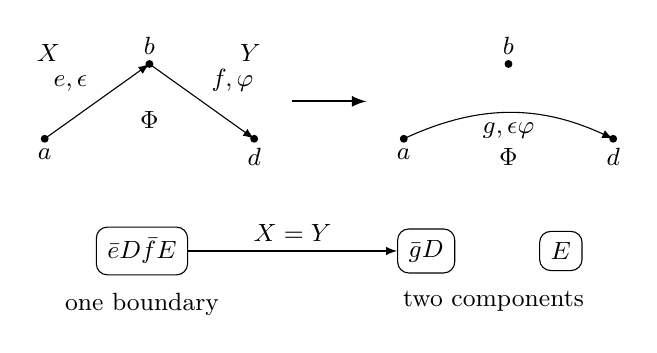
\begin{tikzpicture}[scale=.95,>=latex,every node/.style={font=\small}]
 \coordinate (a) at (-3.8,0);
 \coordinate (b) at (-2.4,1);
 \coordinate (d) at (-1,0);
 \draw[->] (a)--node[above left]{$e,\epsilon$}(b);
 \draw[->] (b)--node[above right]{$f,\varphi$}(d);
 \fill (a) circle (1.5pt) node[below]{$a$};
 \fill (b) circle (1.5pt) node[above]{$b$};
 \fill (d) circle (1.5pt) node[below]{$d$};
 \node at (-2.4,.25) {$\Phi$};
 \node at (-3.75,1.15) {$X$};
 \node at (-1.05,1.15) {$Y$};
 \draw[->,thick] (-.5,.5)--(.5,.5);
 \coordinate (aa) at (1,0);
 \coordinate (bb) at (2.4,1);
 \coordinate (dd) at (3.8,0);
 \draw[->] (aa) to[bend left=25] node[below]{$g,\epsilon\varphi$}(dd);
 \fill (aa) circle (1.5pt) node[below]{$a$};
 \fill (bb) circle (1.5pt) node[above]{$b$};
 \fill (dd) circle (1.5pt) node[below]{$d$};
 \node at (2.4,-.25) {$\Phi$};
 \node[draw,rounded corners,inner sep=4pt] (oldwalk) at (-2.5,-1.5)
   {$\bar eD\bar fE$};
 \node[draw,rounded corners,inner sep=4pt] (newwalk) at (1.3,-1.5)
   {$\bar gD$};
 \node[draw,rounded corners,inner sep=4pt] (otherwalk) at (3.1,-1.5)
   {$E$};
 \draw[->] (oldwalk)--node[above]{$X=Y$}(newwalk);
 \node[below=3pt] at (oldwalk.south) {one boundary};
 \node[below=3pt] at (2.2,-1.8) {two components};
\end{tikzpicture}
\caption{Smoothing two consecutive nonloop darts of one label.
All other incidences are omitted.  The opposite faces $X,Y$ may be
the same face; in that case its boundary splits as shown below the local
picture. The resulting drawing has two components, as the boundary-walk
calculation shows. If $E$ is empty, its component is the isolated vertex $b$.}
\label{fig:gluing-smoothing}
\end{figure}

Across the components, the total number of boundary walks increases
by one, the edge count decreases by one, and the vertex count is
unchanged.  Formula~\eqref{eq:gluing-euler} gives exactly two
components.  The new edge places $a,d$ in one of them.  Every component
must contain an endpoint of a removed edge, because the old graph was
connected; hence $b$ is in the other component.  In particular, the two
walks in~\eqref{eq:gluing-smooth-split} belong to different components.

Give both walks type $j$, and denote their evaluations by
\[
 A=(\epsilon\varphi)^{-1}D,\qquad B=E.
\]
The old word has evaluation $\epsilon^{-1}D\varphi^{-1}B$.
Moving the first factor $\epsilon^{-1}D$ to the end is a cyclic
change of starting point, so it preserves identity versus nonidentity.
The resulting evaluation is
\begin{equation}\label{eq:gluing-split-evaluation}
 (\varphi^{-1}B\varphi)A.
\end{equation}
If $X$ was exceptional, at least one of $A,B$ is nonidentity; retain
its component.  If $X$ was ordinary, $A$ and $B$ are either both
identity or both nonidentity.  In the former case keep the component
with the original exceptional face, whose evaluation is unchanged
even if it is $\Phi$.  In the latter keep the component without that
face; its new boundary is its sole exception.  This again gives a
smaller exceptional map.  We have proved that no face of the minimal
map has consecutive nonloop darts with equal labels, including the
last and first darts of its cyclic boundary walk.

\paragraph{Euler's formula rules out the minimal map.}
Consider a vertex that is not the base of a loop.  Reading the adjacent
face types around it gives a closed walk in $\Delta$.  Each incident
edge crosses between its two different endpoint types, and successive
edge labels are distinct by the smoothing reduction.  Thus the walk
has no immediate reversal.  Its length is positive since the connected
map has edges.  A simple triangle-free graph has no such closed walk
of length less than four, so this vertex has degree at least four.

An ordinary face not incident to a loop has a nonempty boundary walk.
Indeed every boundary walk of a connected graph with at least one
edge is a nonempty dart cycle; an empty walk occurs only for an isolated
vertex.  Its consecutive labels are distinct, and the short-word
condition~\eqref{eq:gluing-short-word} therefore forces its length to
be at least four.  Here and below a loop counts twice toward its
vertex degree, and boundary lengths count dart occurrences.

For our connected spherical map, Euler's formula and the two degree
sums give
\begin{equation}\label{eq:gluing-deficit}
 \sum_{v}(4-\deg v)+\sum_{F}(4-|\partial F|)=8.
\end{equation}
Without a loop, only the exceptional face can contribute positively,
and its nonempty walk contributes at most $3$.  With a loop, its base
vertex contributes at most $2$, the exceptional monogon contributes
$3$, and the face on the other side of the loop contributes at most
$2$: that face is ordinary and cannot have length one, since its sole
letter would be the loop's nonidentity value.  There are no other
loops, so every remaining vertex and face contributes at most zero.
The total is at most $2+3+2=7$, again contradicting
\eqref{eq:gluing-deficit}.  Consequently no exceptional map exists,
and every $D_i^0\to L$ is injective.

\paragraph{Extending to the full vertex groups.}
Let $\Omega=L\times\mathbb N$, with $L$ acting by left multiplication
on the first coordinate.  The restriction to each embedded $D_i^0$
is free and has countably infinitely many orbits.  The same is true
of the left $D_i^0$-action on $D_i\times\mathbb N$.  Pair their orbits
and choose one point in each pair; this determines a $D_i^0$-equivariant
bijection $D_i\times\mathbb N\to\Omega$.  Transport the free left
$D_i$-action along this bijection.  Its restriction to $D_i^0$ is
exactly the original $L$-action.  Make this choice separately for each
$i$.  The resulting actions agree on every edge group because both
copies of its chosen generator act as $x_\gamma\in L$.  They therefore
define an action of $Q$ on $\Omega$, faithful on every $D_i$.  This
proves the required injections.
\end{proof}

\subsection{Application to the modular construction}

Recall from Section~\ref{op:finite-section} the group
$H=A_0\rtimes P$, with $P=(\F_p)^3$ and
$A_0=(\mathbb Z/M\mathbb Z)^P$. Its subgroups
$U=u(P)$ and $V=cUc^{-1}$ satisfy $U\cap V=\{1\}$.
The quotient $G_0$ identifies, for every edge $i<j$, the elements
\begin{equation}\label{eq:gluing-embeddings}
 v(1,\bar j,\bar j^{2})\in H_i,
 \qquad u(1,\bar i,\bar i^{2})\in H_j,
\end{equation}
where $\bar i$ denotes the residue of $i$ in $\mathbb F_p$.
Both elements have order $p$, so the corresponding maps from $C_p$
are embeddings. We now verify the remaining local condition.

\begin{proposition}\label{prop:first-gluing-injective}
Every natural map $H_i\to G_0$ is injective.  In particular, the maps
$K[H_i]\to K[G_0]$ induced on group algebras are injective.
\end{proposition}

\begin{proof}
We verify the short-word hypothesis of
Lemma~\ref{lem:triangle-free-gluing}.  At a fixed vertex, every incident
edge subgroup lies either in $U$ or in $V$.  Within either subgroup,
the labels supplied by distinct neighbors $j$ correspond to the
vectors $(1,\bar j,\bar j^{2})$; a nonidentity syllable corresponds
to a nonzero scalar multiple of its vector.  Any three with distinct residues
are independent, because their determinant is, up to sign,
\[
 (\bar j_2-\bar j_1)(\bar j_3-\bar j_1)
 (\bar j_3-\bar j_2)\neq0.
\]
The residues are distinct since $p>m$.  The analogous first two
coordinates show independence for two vectors, and a single vector
is nonzero.  Thus a word of at most three nonidentity syllables with
distinct labels, all in $U$ or all in $V$, cannot evaluate to $1$.

For a mixed word of length two or three, one of $U,V$ supplies exactly
one syllable.  After a cyclic permutation, a putative relation would
equate that nonidentity syllable to a product of syllables from the
other subgroup. This contradicts $U\cap V=\{1\}$. For lengths
two and three, cyclically distinct consecutive labels are precisely
distinct labels, so all required words have been covered.  The graph
$\Gamma$ is simple and triangle-free, and all groups in question are
finite.  The lemma proves the injections.  The group-algebra assertion
follows because distinct elements of an embedded subgroup remain
distinct basis elements of $K[G_0]$.
\end{proof}

\section{Realizing the local ranks in a common central sector}
\label{sec:sector}

An idempotent in a finite group algebra has a well-defined rank as a
linear operator.  We now turn each of these numerical ranks into an
isomorphism between modules over one common ring.  The enlargement of the
group is needed because the different simple or modular summands of the
original group algebra need not have the same rank fraction.

Here are the precise inputs to this step.  Let $K$ be a field of
characteristic $p$, let $M$ be a positive integer prime to $p$, and assume
that $K$ contains an element $\zeta$ of order $M$.  In the application,
$M=p^4-1$ and $|K|=p^4$. Write $C_M=\mathbb Z/M\mathbb Z$ and put
\[
 P=(\mathbb F_p)^3,\qquad A_0=(C_M)^P,\qquad
 H=A_0\rtimes P,\qquad w=|H|,
\]
where $P$ acts on the functions in $A_0$ by translation. Suppose that a
countable group $G_0$ contains specified copies $H_1,\ldots,H_m$ of $H$.
For each $i$, let $e_i\in K[H_i]$ be an idempotent, and assume that the
positive integer
\[
 d=\dim_K e_iK[H_i]
\]
is independent of $i$.  All matrices below act on column vectors in
free right modules, so their entries multiply coordinates on the left.

\begin{proposition}\label{prop:sector-ranks}
Under these assumptions, there is a group $G_1$ containing $G_0$ and a
central element $z\in G_1$ of order $M$ with the following property.  Set
\[
 R=K[G_1],\qquad
 f=\frac1M\sum_{k=0}^{M-1}\zeta^{-k}z^k,\qquad
 S=fR,\qquad P_i=fe_i.
\]
Then $f$ is a nonzero central idempotent.  There are explicitly
specified matrices
\[
 J_i\in\operatorname{Mat}_{w\times d}(S),\qquad
 Y_i\in\operatorname{Mat}_{d\times w}(S)
\]
satisfying
\begin{equation}\label{eq:sector-rectangular}
 Y_iJ_i=fI_d,\qquad J_iY_i=P_iI_w.
\end{equation}
The entries of $J_i$ and $Y_i$ lie in the group algebra of a finite
subgroup of $G_1$, multiplied by $f$.  Their construction uses only
finite group operations and linear algebra over $K$.
\end{proposition}

We prove the proposition in three stages.  First we attach the finite
groups while preserving all the given embeddings.  Next we describe
their $f$-parts as matrix algebras over group algebras of elementary
abelian $p$-groups.  Finally, nilpotence of the corresponding
augmentation ideals makes the ranks exact and produces the two
rectangular matrices.

\subsection{Attaching the finite groups}

Let $z$ initially generate an independent copy of $C_M$, and write
$Q_{\mathrm{base}}=\langle z\rangle\times G_0$.  For each $i$, define
\[
 B_i=(C_M)^{H_i},\qquad L_i=B_i\rtimes H_i,
 \qquad (h\cdot b)(x)=b(h^{-1}x).
\]
The groups $B_i$ are written additively.  Let $\delta_i\in B_i$ be the
constant function of value $1\in C_M$.  It has order $M$ and is fixed
by $H_i$, so it is central in $L_i$.  Moreover,
$\langle\delta_i\rangle\cap H_i=1$.  Thus
$C_i=\langle z\rangle\times H_i$ embeds in both $Q_{\mathrm{base}}$ and $L_i$, with
$(z^k,h)$ sent to $(k\delta_i,h)$ in the latter.  Define $G_1$ to be
the quotient of the free product
\[
 Q_{\mathrm{base}}*L_1*\cdots*L_m
\]
that identifies these two copies of $C_i$ for every $i$.

For completeness, the following action proves that all the factors
embed in this quotient.  Let $X$ be a countable disjoint union of copies
of the left regular $Q_{\mathrm{base}}$-set.  Its restriction to each $C_i$ is free and
has countably infinitely many orbits.  A countable disjoint union
$X_i$ of regular $L_i$-sets has the same property when restricted to
$C_i$.  Pair their $C_i$-orbits and choose one point in each paired
orbit; extending those point pairings equivariantly gives a
$C_i$-equivariant bijection $X\to X_i$.  Transport the regular
$L_i$-action to $X$ using this bijection.  The resulting actions of
$Q_{\mathrm{base}},L_1,\ldots,L_m$ agree on every prescribed $C_i$, hence define an
action of $G_1$ on $X$.  Each factor acts faithfully, which proves its
injectivity in $G_1$.  This argument uses the assumed embeddings
$H_i\hookrightarrow G_0$ in defining the subgroups $C_i\le Q_{\mathrm{base}}$.

The element $z$ is central in every generating factor of $G_1$ and
therefore in $G_1$; its order is still $M$ because $Q_{\mathrm{base}}$ embeds.
In $R$, direct multiplication gives
\[
 zf=\zeta f,\qquad
 f^2=\frac1M\sum_{k=0}^{M-1}\zeta^{-k}z^kf=f.
\]
The coefficient of the identity in $f$ is $M^{-1}\ne0$, since the
elements $1,z,\ldots,z^{M-1}$ are distinct.  Thus $f$ is a nonzero
central idempotent, and $S=fR$ is a ring with identity $f$.  Each $P_i$
is an idempotent in $fK[L_i]$.  Also, any identity $e_ie_j=0$ already
valid in $K[G_0]$ remains valid after multiplication by $f$ in $S$.

\subsection{The matrix blocks of the central sector}

Fix $i$ for the moment.  A character of $B_i$ means a homomorphism
$\chi:B_i\to K^*$.  If $b_x$ denotes the coordinate function with
value $1$ at $x\in H_i$ and $0$ elsewhere, then every character is
uniquely specified by exponents $a_x\in\mathbb Z/M\mathbb Z$ through
$\chi(b_x)=\zeta^{a_x}$.  Define
\[
 p_\chi=\frac1{|B_i|}\sum_{b\in B_i}\chi(b)^{-1}b
 \quad\text{in }K[B_i].
\]
Apply the Fourier calculation of Equation~\eqref{op:fourier}
to the finite index set $H_i$. The denominator is invertible because
$p\nmid M$. The elements $p_\chi$ are a basis of pairwise orthogonal
idempotents whose sum is $1$, and $bp_\chi=\chi(b)p_\chi$.

Use the action
\[
 (h\chi)(b)=\chi(h^{-1}\cdot b).
\]
Then $hp_\chi h^{-1}=p_{h\chi}$.  Since $z=\delta_i$ is fixed by
$H_i$, the set
\[
 \mathcal X_i=\{\chi:\chi(z)=\zeta\}
\]
is $H_i$-invariant, and the Fourier formulas give
\begin{equation}\label{eq:sector-fourier-f}
 f=\sum_{\chi\in\mathcal X_i}p_\chi.
\end{equation}
For each orbit in $\mathcal X_i$, choose one representative $\theta$
and put $T_\theta=\operatorname{Stab}_{H_i}(\theta)$.

\begin{lemma}\label{lem:sector-stabilizers}
For each such $\theta$, the subgroup $T_\theta$ is elementary abelian
of exponent $p$ and rank at most $3$, with the trivial subgroup allowed.
\end{lemma}

\begin{proof}
Write $\theta(b_x)=\zeta^{a_x}$.  Since
$z=\sum_{x\in H_i}b_x$, the condition on $\theta$ is
\[
 \sum_{x\in H_i}a_x=1\quad\text{in }\mathbb Z/M\mathbb Z.
\]
Suppose that a nonidentity $g\in A_0\cap T_\theta$ has order $q$.
The exponent of $A_0$ divides $M$, so $q>1$ divides $M$. Left
multiplication by $g$ partitions $H_i$ into cycles of length exactly
$q$.  Invariance of $\theta$ says that the exponents $a_x$ are
constant on these cycles.  Their sum consequently lies in
$q(\mathbb Z/M\mathbb Z)$.  It cannot equal $1$: reduction modulo
$q$ would give $0=1$.  This contradiction proves
$T_\theta\cap A_0=1$. The quotient homomorphism
$H_i\to H_i/A_0\cong P$ is therefore injective on $T_\theta$.
Every subgroup of the additive group $(\mathbb F_p)^3$ is an
$\mathbb F_p$-linear subspace, giving the assertion.
\end{proof}

Eliminating the prime-to-$p$ part of each stabilizer is what makes its
augmentation ideal nilpotent, and will permit the later change of basis.
We next give the block isomorphism, including its inverse. This is the
character-orbit construction already used in
Section~\ref{op:modular-section}, now allowing nontrivial stabilizers;
compare the Clifford-theoretic orbit picture in~\cite{Clifford1937Announcement}.
It will identify the underlying $K$-linear rank of $P_i$ in every block
with the same original integer $d$. For one orbit representative
$\theta$, abbreviate
\[
 T=T_\theta,\qquad s=[H_i:T],\qquad D=K[T].
\]
Choose representatives $r_1,\ldots,r_s$ of the left cosets $hT$.
The space $K[H_i]$ is a free right $D$-module with this ordered basis.
Let $g\in H_i$ act on it by left multiplication $L_g$, and let
$b\in B_i$ act diagonally by
\[
 D_b(h)=(h\theta)(b)h\qquad(h\in H_i).
\]
Both actions commute with the right action of $T$.  For the diagonal
action this follows from $(ht)\theta=h\theta$ for $t\in T$.
The semidirect-product relation is also respected, because
\[
 L_gD_bL_g^{-1}(h)
   =((g^{-1}h)\theta)(b)h
   =(h\theta)(g\cdot b)h
   =D_{g\cdot b}(h).
\]
Thus we have an algebra homomorphism
$\rho_\theta:K[L_i]\to\operatorname{Mat}_s(D)$.
The element $z$ acts as $\zeta$, so $\rho_\theta(f)=I_s$.

For $t_0\in T$ and $1\le a,b\le s$, consider
\begin{equation}\label{eq:sector-block-inverse}
 p_{r_a\theta}\,r_at_0r_b^{-1}.
\end{equation}
It belongs to $fK[L_i]$ by \eqref{eq:sector-fourier-f}.  In the
$\theta$-representation it sends $r_bt'$ to $r_at_0t'$ for every
$t'\in T$ and vanishes on every other basis coset.  To check the last
assertion, its left group factor sends the coset $r_cT$ to
$r_at_0r_b^{-1}r_cT$; the Fourier projection keeps this coset precisely
when it equals $r_aT$, which is equivalent to $c=b$.  In a
representation associated to another orbit, the Fourier projection
vanishes identically.  Consequently \eqref{eq:sector-block-inverse}
maps to the matrix with entry $t_0$ in position $(a,b)$ of the
$\theta$-block and zero elsewhere.

Taking the product of these representations gives a surjective map
\begin{equation}\label{eq:sector-blocks}
 \rho:fK[L_i]\longrightarrow
 \prod_{\theta}\operatorname{Mat}_{[H_i:T_\theta]}(K[T_\theta]).
\end{equation}
It is injective as well.  The elements $p_\chi h$, for
$\chi\in\mathcal X_i$ and $h\in H_i$, form a basis of its source.
An orbit of size $s$ contributes $sw=s^2|T|$ basis elements, equal to
the dimension of the corresponding target block.  Hence the source
and target have equal finite $K$-dimension.  Formula
\eqref{eq:sector-block-inverse}, extended linearly in $t_0$ and summed
over the positions and blocks, is an explicit inverse of $\rho$.

\subsection{Turning dimensions into rectangular identities}

Continue in one block and let $E=\rho_\theta(P_i)\in
\operatorname{Mat}_s(D)$.  As a $K$-linear operator on $K[H_i]$,
$E$ is exactly left multiplication by $e_i$, since $f$ acts as the
identity.  Therefore
\begin{equation}\label{eq:sector-regular-rank}
 \dim_K\operatorname{im}E=d.
\end{equation}
This is the link between the original rank calculation and the block
decomposition.  We will now obtain a basis in which $E$ is a coordinate
projection over $D$, not just over $K$. The argument is a constructive
nilpotent-ideal instance of the freeness of projective modules over local
rings, studied by Kaplansky~\cite[Theorem~2]{Kaplansky1958}; no general projective-module
theorem is needed here.

Let $\varepsilon:D\to K$ be augmentation, and set
$\mathfrak a=\ker\varepsilon$.  By Lemma
\ref{lem:sector-stabilizers}, we may choose generators
$t_1,\ldots,t_q$ of $T\cong(C_p)^q$ with $0\le q\le3$.
The elements $X_j=t_j-1$ commute, satisfy $X_j^p=0$, and generate
$\mathfrak a$.  Expanding $t_j=1+X_j$ and counting dimensions gives
\[
 D\cong K[X_1,\ldots,X_q]/(X_1^p,\ldots,X_q^p).
\]
It follows that
\[
 \mathfrak a^{D_{\max}+1}=0,\qquad D_{\max}=3(p-1).
\]
Indeed, a monomial of total degree greater than $q(p-1)$ has an
exponent at least $p$.  This also covers $q=0$, when
$D=K$ and $\mathfrak a=0$.  Matrices with entries in $\mathfrak a$
have the same nilpotence bound under multiplication, because each
entry of a product of $D_{\max}+1$ such matrices lies in
$\mathfrak a^{D_{\max}+1}$.

Put $\overline E=\varepsilon(E)$, applying augmentation entrywise,
and let $d_0=\operatorname{rank}_K\overline E$.  As
$\overline E$ is idempotent, its image and the image of
$I_s-\overline E$ form complementary subspaces of $K^s$.
Scan the columns of $\overline E$ in order and keep each column that
increases their span; then do the same for $I_s-\overline E$.
Build $Q$ by taking the corresponding $d_0$ columns of $E$, followed
by the corresponding $s-d_0$ columns of $I_s-E$.  Its augmentation
$Q_0$ is invertible over $K$.  Regard $Q_0$ as a scalar matrix over
$D$, and set $N=Q_0^{-1}(Q-Q_0)$.  Its entries belong to
$\mathfrak a$, so $N^{D_{\max}+1}=0$.  Since $Q=Q_0(I_s+N)$,
\begin{equation}\label{eq:sector-Q-inverse}
 Q^{-1}=\left(\sum_{k=0}^{D_{\max}}(-N)^k\right)Q_0^{-1}.
\end{equation}
Each of the first $d_0$ columns of $Q$ is fixed by $E$, and every
remaining column is killed by $E$.  Thus, for
$\Pi=\operatorname{diag}(I_{d_0},0)$,
\[
 EQ=Q\Pi,\qquad Q^{-1}EQ=\Pi.
\]
Conjugation by $Q$ preserves $K$-dimension of images.  Comparing with
\eqref{eq:sector-regular-rank} gives the integer equalities
\begin{equation}\label{eq:sector-dimensions}
 d=d_0|T|,\qquad w=s|T|,\qquad wd_0=sd.
\end{equation}
In particular, these are equalities of ordinary dimensions, not
equalities after reduction to $K$.

We can now match coordinates exactly.  Order pairs lexicographically
and choose the increasing bijection between
\[
 \{(\mu,l):1\le\mu\le d,\ 1\le l\le s\}
 \quad\text{and}\quad
 \{(\lambda,k):1\le\lambda\le w,\ 1\le k\le d_0\};
\]
the sets have equal size by \eqref{eq:sector-dimensions}.
Let $V$ be the $w$-by-$d$ block matrix with $s$-by-$s$ entries
that sends coordinate $(\mu,l)$ to its paired coordinate
$(\lambda,k)$.  Thus $V_{\lambda\mu}$ is the sum of standard
matrix units $E_{kl}^{\mathrm{std}}$ over all such pairings.
Let $W$ be the $d$-by-$w$ block matrix reversing each pairing, with
$W_{\mu\lambda}$ the corresponding sum of
$E_{lk}^{\mathrm{std}}$.  It sends all unpaired coordinates with
$k>d_0$ to zero.  Directly on these coordinates,
\[
 WV=I_d\otimes I_s,\qquad VW=I_w\otimes\Pi.
\]
Define block matrices
\[
 J^{(\theta)}=(I_w\otimes Q)V,\qquad
 Y^{(\theta)}=W(I_w\otimes Q^{-1}).
\]
They have outer shapes $w\times d$ and $d\times w$, respectively,
with entries in $\operatorname{Mat}_s(D)$.  Their products are
\[
 Y^{(\theta)}J^{(\theta)}=I_d\otimes I_s,\qquad
 J^{(\theta)}Y^{(\theta)}=I_w\otimes E.
\]
Finally define the $(\lambda,\mu)$ entry of $J_i$ by applying
$\rho^{-1}$ to the tuple
$(J^{(\theta)}_{\lambda\mu})_\theta$, and similarly define $Y_i$
entrywise from the $Y^{(\theta)}$.  The isomorphism
\eqref{eq:sector-blocks} carries $f$ to the tuple of identity
matrices and $P_i$ to the tuple of matrices $E$.  The last two
identities therefore pull back to
\eqref{eq:sector-rectangular}.  This proves Proposition
\ref{prop:sector-ranks}.

All choices in the matrix construction are over finite sets: character orbits, coset
representatives, augmentation matrices, and coordinate pairings.
Taking the first element or the first independent columns in fixed
orders makes the prescription definite.  The inverse
\eqref{eq:sector-Q-inverse} is a finite sum, and the inverse
\eqref{eq:sector-block-inverse} is a finite group-algebra formula.
Thus the matrices furnished by the proposition are finite sums in
the explicitly attached finite groups.

We now apply Proposition~\ref{prop:sector-ranks} to the embedded groups
of Proposition~\ref{prop:first-gluing-injective} and the identical
idempotents of Proposition~\ref{op:modular}. The group $G_0$
is countable because it is finitely generated. All the ranks equal the
positive integer $d$ from Equation~\eqref{op:regular-rank}.
Hence the group $G_1$, the nonzero central idempotent $f$, and the
matrices $J_i,Y_i$ are now fixed by the constructions above.
Corollary~\ref{op:edge-zero} also gives $P_iP_j=0$ on every
edge with $i<j$. These are precisely the inputs to the next section.

\section{Compression with a visible nonzero defect}
\label{op:compression-section}

We now use only the graph factorization and the precise common-sector
output. The first lemma is independent of the group construction. Its
proof explains why ordered edge annihilations, rather than symmetric
orthogonality, suffice.

\begin{lemma}[Triangular compression]\label{op:compression}
Let $S$ be a nonzero unital algebra over a field $K$, and let $m,t,w,d$
be positive integers. Suppose $P_i\in S$ are idempotents and
$\alpha_i(T),\beta_j(T)\in K$ satisfy
\[
 F_{ij}=\sum_{T=1}^t\alpha_i(T)\beta_j(T),\qquad
 F_{ii}=1,\qquad F_{ij}P_iP_j=0\quad(i<j).
\]
Suppose there are $J_i\in\Mat_{w\times d}(S)$ and
$Y_i\in\Mat_{d\times w}(S)$ with
$Y_iJ_i=I_d$, $J_iY_i=P_iI_w$. Then explicit matrices
\[
 C_\sharp\in\Mat_{wt\times md}(S),\qquad
 D_\sharp\in\Mat_{md\times wt}(S)
\]
satisfy $D_\sharp C_\sharp=I_{md}$.
\end{lemma}
\begin{proof}
Define $C_0$ of shape $t\times m$ and $D_0$ of shape $m\times t$ by
\[
 (C_0)_{T,j}=\beta_j(T)P_j,\qquad
 (D_0)_{i,T}=\alpha_i(T)P_i.
\]
Their product has entries $F_{ij}P_iP_j$. Therefore
$D_0C_0=\mathcal P+\mathcal N$, where
$\mathcal P=\diag(P_1,\ldots,P_m)$ and $\mathcal N$ is strictly
lower triangular. In particular $\mathcal N^m=0$. Every off-diagonal
entry begins with $P_i$ and ends with $P_j$, so idempotence gives
\[
 \mathcal P^2=\mathcal P,\qquad
 \mathcal P\mathcal N=\mathcal N=\mathcal N\mathcal P.
\]
This is all the commutation information needed. The finite sum
\[
 \mathcal Q=\mathcal P+\sum_{k=1}^{m-1}(-\mathcal N)^k
\]
satisfies $\mathcal Q(\mathcal P+\mathcal N)=\mathcal P$ by cancellation
of consecutive powers. Put $D_1=\mathcal QD_0$; then
$D_1C_0=\mathcal P$. For $m=1$ the sum is empty and the same identity
holds.

Take block diagonals $C_{\rm rep}$ and $D_{\rm rep}$ of $w$ copies
of $C_0$ and $D_1$. Use ordered coordinates $(\lambda,i)$ on $S^{wm}$
and $(\lambda,T)$ on $S^{wt}$. Their product is
\[
 D_{\rm rep}C_{\rm rep}=\mathcal P_{\rm rep}
 :=\diag_{\lambda=1}^w(\mathcal P).
\]
Define matrices $\mathcal J:S^{md}\to S^{wm}$ and
$\mathcal Y:S^{wm}\to S^{md}$ by
\[
 \mathcal J_{(\lambda,i),(j,\mu)}
     =\delta_{ij}(J_i)_{\lambda\mu},\qquad
 \mathcal Y_{(j,\mu),(\lambda,i)}
     =\delta_{ij}(Y_i)_{\mu\lambda},
 \quad 1\le\mu\le d.
\]
The assumed rectangular identities give
$\mathcal Y\mathcal J=I_{md}$ and
$\mathcal J\mathcal Y=\mathcal P_{\rm rep}$. Thus
\[
 C_\sharp=C_{\rm rep}\mathcal J,\qquad
 D_\sharp=\mathcal YD_{\rm rep}
\]
have the asserted shapes and satisfy
\[
 D_\sharp C_\sharp
 =\mathcal Y\mathcal P_{\rm rep}\mathcal J
 =\mathcal Y\mathcal J\mathcal Y\mathcal J=I_{md}.
\]
Only associativity and the stated identities have been used; the $P_i$
are not assumed to commute.
\end{proof}

Apply the lemma to $S=fK[G_1]$, whose identity is $f$. Distinct
nonedges have $F_{ij}=0$ by Proposition~\ref{op:graph}; edges with
$i<j$ have $P_iP_j=0$. The rectangular identities are exactly those
of Proposition~\ref{prop:sector-ranks}. Consequently
\begin{equation}\label{op:split}
 D_\sharp C_\sharp=fI_{md},\qquad
 C_\sharp:S^{md}\longrightarrow S^{wt}.
\end{equation}
The strict, ordinary rational inequalities are
\[
 \frac t m<\frac1{100}<\frac1{96}<\frac d w,\qquad
 r:=wt<md=:N.
\]
This is more than an abstract rank paradox: it gives a nonzero vector
that will certify the reverse-product defect.

\begin{lemma}[A square inverse and its certificate]\label{op:kernel}
Let $R$ be a unital ring, $f\ne0$ a central idempotent, and $S=fR$.
Suppose $N>r\ge1$ and matrices
$C\in\Mat_{r\times N}(S)$, $D\in\Mat_{N\times r}(S)$ satisfy
$DC=fI_N$. Let $\iota:S^r\to S^N$ include the first $r$ coordinates
and $\pi:S^N\to S^r$ retain them, with entries $f$ and zero. Then
\[
 A_R=\pi D+(1-f)I_r,\qquad B_R=C\iota+(1-f)I_r
\]
satisfy $A_RB_R=I_r$ and $B_RA_R\ne I_r$. More precisely, if
$u_*\in S^N$ has last coordinate $f$ and all others zero, then
\[
 v_*:=Cu_*\ne0,\qquad Dv_*=u_*,\qquad
 A_Rv_*=0,\qquad (B_RA_R-I_r)v_*=-v_*\ne0.
\]
\end{lemma}
\begin{proof}
Every entry of $C,D,\iota,\pi$ belongs to $S$ and is annihilated on
both sides by $1-f$. Since $\pi\iota=fI_r$,
\[
 A_RB_R=\pi DC\iota+(1-f)I_r=fI_r+(1-f)I_r=I_r.
\]
The vector $u_*$ is nonzero because $f\ne0$. The equation
$Dv_*=DCu_*=u_*$ proves $v_*\ne0$. But $N>r$ makes
$\pi u_*=0$, so
\[
 A_Rv_*=\pi Dv_*+(1-f)v_*=0.
\]
Multiplying by $B_R$ and subtracting $v_*$ gives the final displayed
identity and proves the strict reversal defect.
\end{proof}

Using $C=C_\sharp$, $D=D_\sharp$ in Lemma~\ref{op:kernel} gives
square matrices over the entire algebra $K[G_1]$, not only the
$f$-summand. The nonzero certificate is rooted in the exact order of
$z$, which proves $f\ne0$, and then in $D_\sharp v_*=u_*$. It does
not depend on identifying a coefficient by deciding equality of group
words. The remaining step is to retain this defect when replacing
matrices by scalar elements.

\section{An injective finite-group encoding}
\label{op:scalar-section}

We have a strict matrix one-sided inverse over $K[G_1]$. The
finite-factor reduction of Dykema and Juschenko
\cite[Lemma~2.1 and Theorem~2.2]{DykemaJuschenko2015} explains the
appropriate next step: put a full matrix algebra inside a finite group
algebra and fill the complementary summand with the identity. We prove
the actual matrix block needed here, including its injectivity. Its
shift and diagonal operators are the finite Heisenberg model; the
comparison with~\cite[Section~1.2]{GurevichHadani2009} is methodological,
since our cyclic order can be composite and our coefficient field is
finite.

\begin{proposition}\label{op:heisenberg}
Let $K$ be a field, let $M\ge2$ be invertible in $K$, and let
$\zeta\in K$ have order $M$. For an integer $q\ge0$ put
$Z_q=(\mathbb Z/M\mathbb Z)^q$ and $n=M^q$. There is a finite group
$\Lambda$ of order $Mn^2$ and a nonzero central idempotent
$f'\in K[\Lambda]$ for which explicitly specified elements
$\Omega_{uv}$, $u,v\in Z_q$, form a basis of $f'K[\Lambda]$ and obey
\[
 \Omega_{uv}\Omega_{st}=\delta_{vs}\Omega_{ut},\qquad
 \sum_u\Omega_{uu}=f'.
\]
Thus $\Mat_n(K)\cong f'K[\Lambda]$ by its standard matrix units.
\end{proposition}
\begin{proof}
Use the set $\Lambda=Z_q\times Z_q\times\mathbb Z/M\mathbb Z$ with
\begin{equation}\label{op:heisenberg-law}
 (x,y,k)(x',y',k')=(x+x',y+y',k+k'+y\cdot x').
\end{equation}
All coordinates and the dot product use residues modulo $M$.
Associativity follows from the bilinear identity
\[
 y\cdot x'+(y+y')\cdot x''=y'\cdot x''+y\cdot(x'+x'').
\]
The zero tuple is the identity, and the inverse is
$(-x,-y,-k+y\cdot x)$. No primality of $M$ is involved.
The element $z'=(0,0,1)$ is central of exact order $M$. Define
\[
 f'=\frac1M\sum_{k=0}^{M-1}\zeta^{-k}(z')^k.
\]
Reindexing gives $z'f'=\zeta f'$, and convolution gives $(f')^2=f'$.
The identity coefficient $M^{-1}$ is nonzero, so $f'\ne0$.

Write $X_x=(x,0,0)$ and $Y_y=(0,y,0)$, and put
\begin{equation}\label{op:heisenberg-D}
 D_v=\frac1n\sum_{y\in Z_q}\zeta^{-y\cdot v}f'Y_y.
\end{equation}
The denominator is invertible because $n=M^q$. Character orthogonality
here means the direct identity
\begin{equation}\label{op:composite-orthogonality}
 \sum_{y\in Z_q}\zeta^{y\cdot a}
 =\begin{cases}n,&a=0,\\0,&a\ne0.\end{cases}
\end{equation}
When $a\ne0$, choose a nonzero coordinate $a_j$. Translation of the
sum by the $j$th coordinate vector multiplies it by
$\zeta^{a_j}\ne1$. In the field $K$, this forces the sum to vanish.
The argument still works when $a_j$ is a zero divisor modulo the
composite integer $M$.

Convolution in the abelian group of $Y_y$ gives
$D_vD_t=\delta_{vt}D_t$; indeed the coefficient of $f'Y_b$ in the
product is
\[
 \frac{\zeta^{-b\cdot t}}{n^2}
       \sum_{y\in Z_q}\zeta^{y\cdot(t-v)}.
\]
Summing Equation~\eqref{op:heisenberg-D} over $v$ also gives
$\sum_vD_v=f'$. The group law gives
$Y_yX_a=(z')^{y\cdot a}X_aY_y$, and hence
\[
 D_vX_a=X_aD_{v-a}.
\]
Set
\begin{equation}\label{op:matrix-units}
 \Omega_{uv}=X_{u-v}D_v
 =X_{u-v}\frac1n\sum_{y\in Z_q}\zeta^{-y\cdot v}f'Y_y.
\end{equation}
Then
\[
 \Omega_{uv}\Omega_{st}
 =X_{u-v+s-t}D_{v-s+t}D_t
 =\delta_{vs}\Omega_{ut},
\]
and the diagonal sum is $f'$.

The multiplication identities alone do not yet prove that this block
has no kernel. On $K^{Z_q}$ define
\[
 \rho(x,y,k)\mathbf e_s=\zeta^{k+y\cdot s}\mathbf e_{s+x}.
\]
The scalar in a composite is
$\zeta^{k+k'+y\cdot x'+(y+y')\cdot s}$, so
Equation~\eqref{op:heisenberg-law} proves that $\rho$ is a representation.
It sends $f'$ to the identity and $D_v$ to the coordinate projection
at $v$. Therefore
\[
 \rho(\Omega_{uv})\mathbf e_s=\delta_{vs}\mathbf e_u,
\]
which proves independence of all $n^2$ elements $\Omega_{uv}$.
On the other hand, the $n^2$ elements $f'(x,y,0)$ span $f'K[\Lambda]$,
because $f'(x,y,k)=\zeta^k f'(x,y,0)$. Their group-basis supports have
distinct $(x,y)$ coordinates, so they too are independent. The sector
has dimension exactly $n^2$, and the matrix units form a basis.
When $q=0$, the empty tuple set has one element: $n=1$, $\Lambda=C_M$,
and the sole matrix unit is $f'$. All formulas remain valid.
\end{proof}

The elementary identity-completion step is worth recording separately.
Its unit need not be central in the target ring.

\begin{lemma}\label{op:complement}
Let $\Phi:\mathcal A\to\mathcal B$ be an injective ring homomorphism
between unital rings, not necessarily preserving their identities, and
put $g=\Phi(1_{\mathcal A})$. If $AB=1_{\mathcal A}$ and
$BA\ne1_{\mathcal A}$, then
\[
 a=1_{\mathcal B}-g+\Phi(A),\qquad
 b=1_{\mathcal B}-g+\Phi(B)
\]
satisfy $ab=1_{\mathcal B}$ and $ba\ne1_{\mathcal B}$.
\end{lemma}
\begin{proof}
The element $g$ is idempotent and is an identity on the image of $\Phi$
on both sides. Thus $1-g$ annihilates that image on both sides. Expanding
the two products gives
\[
 ab=1-g+\Phi(AB)=1,\qquad
 ba-1=\Phi(BA-1)\ne0.
\]
Only the last inequality uses injectivity; no global centrality of $g$
is required.
\end{proof}

\begin{corollary}\label{op:scalar}
Under the field hypotheses of Proposition~\ref{op:heisenberg}, suppose
$A,B\in\Mat_r(K[L])$ for a group $L$ and an integer $r\ge1$, with
$AB=I_r$ and $BA\ne I_r$. Finite formulas give a finite group $\Lambda$
and $a,b\in K[L\times\Lambda]$ with $ab=1$ and $ba\ne1$.
In particular, over any fixed finite field with at least three elements,
a failure of stable finiteness transfers to a scalar failure after a
finite direct factor, without changing the field.
\end{corollary}
\begin{proof}
Choose the least $q\ge0$ with $n=M^q\ge r$. This search is finite,
since $M^r\ge2^r\ge r$. Pad the matrices by identities:
\[
 \widetilde A=\diag(A,I_{n-r}),\qquad
 \widetilde B=\diag(B,I_{n-r}).
\]
The padding is empty if $n=r$. Then
$\widetilde A\widetilde B=I_n$ and
$\widetilde B\widetilde A-I_n=\diag(BA-I_r,0)\ne0$.
Use Proposition~\ref{op:heisenberg} and the group-basis identification
$K[L\times\Lambda]=K[L]\otimes_K K[\Lambda]$. For an $n$-square
matrix $T$ over $K[L]$, put
\[
 \Phi(T)=\sum_{u,v\in Z_q}T_{uv}\otimes\Omega_{uv}.
\]
The matrix-unit products prove multiplicativity, with
$\Phi(I_n)=1\otimes f'$. Independence of the $\Omega_{uv}$ gives
injectivity: extend their coordinate dual functionals to $K[\Lambda]$
and apply each in the second tensor factor to recover $T_{uv}$.
This works even when $K[L]$ has zero divisors.

Lemma~\ref{op:complement} now yields the promised finite sums
\begin{equation}\label{op:scalar-formulas}
 \begin{split}
 a&=1\otimes(1-f')+
       \sum_{u,v\in Z_q}\widetilde A_{uv}\otimes\Omega_{uv},\\
 b&=1\otimes(1-f')+
       \sum_{u,v\in Z_q}\widetilde B_{uv}\otimes\Omega_{uv}.
 \end{split}
\end{equation}
Their full scalar product is one, and their reverse defect is
$\Phi(\widetilde B\widetilde A-I_n)\ne0$.
For a finite field of order $Q\ge3$, take $M=Q-1$ and a generator
of its multiplicative group. Then $M\ge2$ is invertible in the field,
so the preceding construction applies.
\end{proof}

\begin{proof}[Proof of Theorem~\ref{op:main}]
Lemma~\ref{op:field} supplies the specified odd prime and field of
order $p^4$. Propositions~\ref{op:graph} and~\ref{op:modular} give the
graph fit and the strict regular-rank comparison.
Proposition~\ref{prop:first-gluing-injective} embeds the local groups
in $G_0$, and Proposition~\ref{prop:sector-ranks} places their ranks in
the nonzero ring $fK[G_1]$ with the required rectangular identities.
Corollary~\ref{op:edge-zero} supplies every ordered edge product.
Lemmas~\ref{op:compression}
and~\ref{op:kernel} produce $A_R,B_R\in\Mat_r(K[G_1])$, with their
nonzero certificate. Corollary~\ref{op:scalar}, using $L=G_1$ and
$M=p^4-1$, gives $G=G_1\times\Lambda$ and the sums
in Equation~\eqref{op:scalar-formulas}. Their product is one and their
reverse-product defect is nonzero by the injectivity of the matrix
encoding.

The group $G_0$ is generated by the finite groups $H_i$. The construction
of $G_1$ adds only $\langle z\rangle$ and the finitely many finite
groups $L_i$, and $\Lambda$ is finite. Thus $G$ is finitely generated.
The embedded copy of any $H_i$ supplies nontrivial torsion. All field,
group and coefficient choices were given by finite formulas and fixed
orders, as required.
\end{proof}

\paragraph{Finite prescriptions and scope.}
Every choice of character, basis, field element, or finite inverse
occurs in an explicitly finite set. Products of the resulting group
words define finite group-algebra sums even when different words happen
to coincide. No word comparisons are needed to define the elements,
and the kernel certificate and injective matrix block certify the
nonzero reverse defect. The countable permutation actions used to
certify group embeddings are not coefficient-search inputs.

Containing torsion does not say that every element has finite order.
The group must
be infinite, since finite-dimensional left multiplication proves direct
finiteness for every finite group algebra, in modular characteristic as
well as otherwise. The coefficient field throughout remains the
specified $K$ of order $p^4$.

More generally, the supports of any two finite sums in a group algebra
generate a finitely generated subgroup. Its group algebra embeds by the
group bases, preserving both a one-sided product and its nonzero reverse
defect. Thus a universal direct-finiteness theorem for finitely generated
groups would already imply the assertion for all groups.

\section{The cellular automaton on all configurations}
\label{op:cellular-section}

The final transfer is short and characteristic-independent. We give it
locally to fix the multiplication order and the meaning of a missing
configuration. Its group-ring ancestry appears in
\cite[Section~1]{ElekSzabo2004} and the linear theory
of~\cite{CSCCoornaert2006}.

For any field $k$, group $L$, and finite sum $c=\sum_uc_u u\in k[L]$,
define on all functions $x:L\to k$
\[
 (T_cx)(g)=\sum_uc_u x(gu).
\]
Only the coefficient sum is finite; $x$ may have infinite support.
Expanding the two finite sums gives
\begin{equation}\label{op:cellular-product}
 (T_cT_dx)(g)=\sum_{u,v}c_ud_vx(guv)=(T_{cd}x)(g).
\end{equation}
Thus $T_cT_d=T_{cd}$ and $T_1=\id$. If $\delta_h$ is the point
indicator at $h$, then $(T_c\delta_h)(1_L)=c_h$, which also proves
faithfulness.

\begin{proposition}\label{op:cellular}
Let $k$ be a finite field, $L$ a group, and $a,b\in k[L]$ with $ab=1$.
Then $T_b:k^L\to k^L$ is an injective cellular automaton, with
\[
 \im T_b=\{y\in k^L:T_{ba}y=y\}.
\]
For every $h$ with $(ba-1)_h\ne0$, the configuration $\delta_h$ is
absent from its image.
\end{proposition}
\begin{proof}
The support of $b$ is a finite memory set with rule
$(x_u)_u\mapsto\sum_u b_ux_u$. Equation~\eqref{op:cellular-product}
gives $T_aT_b=T_{ab}=\id$, proving injectivity. If $y=T_bx$, then
$T_{ba}y=T_bT_aT_bx=y$. Conversely, a fixed point of $T_{ba}$ has
$y=T_b(T_ay)$, hence lies in the image. Finally,
\[
 (T_{ba}\delta_h-\delta_h)(1_L)=(ba-1)_h\ne0,
\]
so $\delta_h$ is not a fixed point and cannot be in the image.
\end{proof}

Apply the proposition to the scalar sums in
Equation~\eqref{op:scalar-formulas}. Their nonzero defect has a
nonzero coefficient in the group basis, so the resulting automaton is
injective and nonsurjective. The missing point indicator has no
preimage even among infinitely supported configurations. If the finite
formula for $b$ displays a group element more than once, its terms
simply add in the same local rule; specifying the rule requires no
word-problem oracle.
Thus the constructed group also gives a negative answer to Gottschalk's
surjunctivity conjecture.

\begingroup
\raggedright
\bibliographystyle{alphaurl}
\bibliography{references}
\endgroup
\end{document}
